\chapter{Classification \label{chapter:classification}}
One of the earliest application of artificial intelligence is 
\href{https://en.wikipedia.org/wiki/Statistical_classification}{classification}.  A good
example of classification is \href{https://en.wikipedia.org/wiki/Anti-spam_techniques#Detecting_spam}{spam detection}.
A system for spam detection classifies an email as either spam or not spam, where ``not spam'' is often
abbreviated as ``ham''.  To do so, it first
computes various \blue{features} of the email and then uses these features to determine whether the email is
likely to be spam.  For example, a possible feature would be the number of occurrences of the word
``\texttt{pharmacy}'' in the text of the email.

\section{Introduction}
Formally, the \blue{classification problem} in machine learning can be stated as follows:  We are given a
set of objects $S := \{ o_1, \cdots, o_n \}$ and a set of classes $C := \{ c_1, \cdots, c_k \}$.  Furthermore, there exists a function 
\\[0.2cm]
\hspace*{1.3cm}
$\mathtt{classify}: S \rightarrow C$
\\[0.2cm]
that assigns a class $\texttt{classify}(o)$ to every object $o \in S$.  The set $S$ is called the \blue{sample space}.
In the example of spam detection, the sample space $S$ is the set of all emails that we might receive, i.e.~$S$
is the set of all strings, while the set of classes $C$ is given as
\\[0.2cm]
\hspace*{1.3cm}
$C = \{ \mathtt{spam}, \mathtt{ham} \}$.
\\[0.2cm]
Our goal is to compute the function \texttt{classify}.  In order to do this, we use an approach known as
\href{https://en.wikipedia.org/wiki/Supervised_learning}{supervised learning}:  We take a subset $S_\textsl{train} \subseteq S$ of
emails where we already know whether the emails are spam or not.  This set $S_\textsl{train}$ is called the \blue{training set}.
Next, we define a set of $D$ \blue{features} for every $o \in S$.  These features have to be \blue{computable},
i.e.~we must have a function
\\[0.2cm]
\hspace*{1.3cm}
$\mathtt{feature}: S \times \{ 1, \cdots, D \} \rightarrow \mathbb{R}$ 
\\[0.2cm]
such that $\mathtt{feature}(o, j)$ computes the $j$-th feature and we have to be able to implement
this function with reasonable efficiency.  In general, the values of the features are real values.
However, there are cases where these values are just 
Booleans.  If
\\[0.2cm]
\hspace*{1.3cm}
$\texttt{feature}(o, j) \in \mathbb{B}$ \quad for all $o \in S$,
\\[0.2cm]
then the $j$-th feature is called a \blue{binary feature}.  If we encode $\mathtt{false}$ as $-1$ and $\mathtt{true}$ as
$+1$, then the set of Boolean values $\mathbb{B}$ can be considered a subset of $\mathbb{R}$ and hence Boolean features can be considered
as real numbers.  For example, in the case of spam detection, the first feature
could be the occurrence of the string ``\texttt{pharmacy}''.  In this case, we would have
\\[0.2cm]
\hspace*{1.3cm}
$\texttt{feature}(o, 1) := \left\{
\begin{array}{ll}
  +1 & \mbox{if \ $\texttt{pharmacy}     \in o$,}      \\
  -1 & \mbox{if \ $\texttt{pharmacy} \not\in o$,}  
\end{array}\right.
$
\\[0.2cm]
i.e.~the first feature would be to check whether the email $o$ contains the string ``\texttt{pharmacy}''.  
If we want to be more precise, we can instead define the first feature as
\\[0.2cm]
\hspace*{1.3cm}
$\texttt{feature}(o, 1) := \mathtt{count}(\texttt{"pharmacy"}, o)$,
\\[0.2cm]
i.e.~we would count the number of occurrences of the string ``\texttt{pharmacy}'' in our email $o$.   
As the value of
\\[0.2cm]
\hspace*{1.3cm}
 $\mathtt{count}(\texttt{"pharmacy"}, o)$ 
\\[0.2cm]
is always a natural number, in this case the first feature would be a
 \blue{discrete} feature.  However, we can be even more precise: Instead of just counting the number of occurrences of
 ``\texttt{pharmacy}'' we can compute its \blue{frequency}.  After all, there is a difference whether the
 string ``\texttt{pharmacy}'' occurs once in an email  containing but a hundred characters or whether is occurs
 once in an email with a length of several thousand  characters.  To this end, we would then define the first feature as
\\[0.2cm]
\hspace*{1.3cm}
$\ds \texttt{feature}(o, 1) := \frac{\mathtt{count}(\texttt{"pharmacy"}, o)}{\cnt o}$, 
\\[0.2cm]
where $\cnt o$ defines the number of characters in the string $o$.  In this case, the first feature would be a
\blue{continuous} feature and as this is the most general case, unless stated otherwise, we deal with the continuous
case. 

Having defined the features, we next need a \blue{model} of the function \texttt{classify} that tries to approximate the
function \texttt{classify} via the features.  This model is given by a function
\\[0.2cm]
\hspace*{1.3cm}
$\mathtt{model}: \mathbb{R}^D \rightarrow C$
\\[0.2cm]
such that
\\[0.2cm]
\hspace*{1.3cm}
$\mathtt{model}\bigl(\mathtt{feature}(o,1), \cdots, \mathtt{feature}(o,D)\bigr) \approx \mathtt{classify}(o)$.
\\[0.2cm]
Using the function \texttt{model}, we can then approximate the function classify using a function \texttt{guess} that is
defined as
\\[0.2cm]
\hspace*{1.3cm}
$\mathtt{guess}(o) := \mathtt{model}\bigl(\mathtt{feature}(o,1), \cdots, \mathtt{feature}(o,D)\bigr)$
\\[0.2cm]
Most of the time, the function \texttt{guess} will only \blue{approximate} the function \texttt{classify}, i.e.~we will have
\\[0.2cm]
\hspace*{1.3cm}
$\mathtt{guess}(o) = \mathtt{classify}(o)$
\\[0.2cm]
for most objects of $o \in S$ but not for all of them.  The \blue{accuracy} of our model is defined as the fraction
of those objects that are classified correctly, i.e.~
\\[0.2cm]
\hspace*{1.3cm}
$\ds \mathtt{accuracy} := \frac{\;\cnt \{ o \in S \mid \mathtt{guess}(o) = \mathtt{classify}(o)\}\;}{\cnt S}$.
\\[0.2cm]
If the set $S$ is infinite, this equation has to be interpreted as a limit, i.e.~we can define
$S_n$ as the set of strings that have a length of at most $n$.  Then, the accuracy can be defined as a limit:
\\[0.2cm]
\hspace*{1.3cm}
$\ds \mathtt{accuracy} := \lim\limits_{n\rightarrow\infty}\frac{\;\cnt \{ o \in S_n \mid \mathtt{guess}(o) = \mathtt{classify}(o)\}\;}{\cnt S_n}$.
\\[0.2cm]
The function $\mathtt{model}$ is usually determined by a set of \blue{parameters} or \blue{weights} $\mathbf{w}$. In
this case, we have
\\[0.2cm]
\hspace*{1.3cm}
$\mathtt{model}(\mathbf{x}) = \mathtt{model}(\mathbf{x},\,\mathbf{w})$
\\[0.2cm]
where $\mathbf{x}$ is the vector of features, while $\mathbf{w}$ is the vector of weights.  Later, when we
introduce \blue{logistic regression}, we will assume that the number of weights is one more than the number of
features.  Then, the weights specify the relative importance of the different features. Furthermore, there will
be a weight that is interpreted as a \blue{bias term}.

When it comes to the choice of model, it is important to understand that, at least in practical applications,
\underline{all} models are wrong.  Nevertheless, \underline{some} models are useful.  There are two reasons for this:
\begin{enumerate}
\item We do not fully understand the function \texttt{classify} that we want to approximate by the function $\mathtt{model}$.
\item The function \texttt{classify} is so complex, that even if we could compute it exactly, the resulting model 
      would be much too complicated.
\end{enumerate}
The situation is similar in physics: Let us assume that we intend to model the fall of an object.  A model that is a
hundred percent accurate would have to include the following forces:
\begin{enumerate}[(a)]
\item gravitational acceleration,
\item air friction, 
\item tidal forces, i.e.~the effects that the rotation of the earth has on moving objects,
\item celestial forces, i.e.~the gravitational acceleration caused by celestial objects like the moon or the
      sun.
\item In the case of a metallic object we have to be aware of the magnetic forces
      caused by the \href{https://www.britannica.com/science/geomagnetic-field}{geomagnetic field}.
\item To be fully accurate, we might have to include corrections from relativistic physics and even quantum
      physics.   
\item As physics is not a closed subject, there might be other forces at work which we still do not know of. 
\end{enumerate}
Hence, a correct model would be so complicated that it would be unmanageable and therefore useless. 

Let us summarize our introductory discussion of machine learning in general and classification in particular.
A set $S$ of objects and a set $C$ of classes are given.  Our goal is to approximate a function
\\[0.2cm]
\hspace*{1.3cm}
$\mathtt{classify}: S \rightarrow C$
\\[0.2cm]
using certain \blue{features} of our objects.  The function $\mathtt{classify}$ is then approximated using a function
\texttt{model} as follows:
\\[0.2cm]
\hspace*{1.3cm}
$\mathtt{model}\bigl(\mathtt{feature}(o,1), \cdots, \mathtt{feature}(o,D), \mathbf{w}\bigr) \approx \mathtt{classify}(o)$.
\\[0.2cm]
The model depends on a vector of parameters $\mathbf{w}$.  In order to \blue{learn} these parameters, we are given a 
\blue{training set} $S_\textsl{train}$ that is a subset of $S$.  As we are dealing with \blue{supervised learning}, the function 
$\mathtt{classify}$ is known for all objects $o \in S_\textsl{train}$.   Our goal is to determine the parameters $\mathbf{w}$ such that the
number of mistakes we make on the training set is minimized.  

\subsection{Notation}
We conclude this introductory section by fixing some notation.  Let us assume that the objects $o \in S_\textsl{train}$
are numbered 
from $1$ to $N$, while the features are numbered from $1$ to $D$.  Then we define
\begin{enumerate}
\item $\textbf{x}_i := \langle\mathtt{feature}(o_i, 1), \cdots, \mathtt{feature}(o_i, D)\rangle$ \quad for all $i \in \{1, \cdots, N\}$.
  
      i.e.~$\mathbf{x}_i$ is a $D$-dimensional row vector that collects the features of the $i$-th training object.
\item $x_{i,j} := \mathtt{feature}(o_i, j)$ \quad for all $i \in \{1, \cdots, N\}$ and $j \in \{1, \cdots, D\}$.

      i.e.~$x_{i,j}$ is the $j$-th feature of the $i$-th object.
\item $y_i := \mathtt{classify}(o_i)$ \quad for all $i \in \{1, \cdots, N\}$

      i.e.~$y_i$ is the class of the $i$-th object.
\end{enumerate}
Mathematically, our goal is to maximize the accuracy of our model as a function of the parameters $\mathbf{w}$.

\subsection{Applications of Classification}
Besides spam detection, there are many other classification problems that can be solved using machine learning.  To give
just one more example, imagine a general practitioner that receives a patient and examines her symptoms.  In this case,
the symptoms can be seen as the features of the patient.  For example, these features could be
\begin{enumerate}[(a)]
\item body temperature,
\item blood pressure,
\item heart rate,
\item body weight,
\item breathing difficulties,
\item age,
\end{enumerate}
to name but a few of the possible features.  Based on these symptoms, the general practitioner would then decide on an
illness, i.e.~the set of classes for the classification problem would be
\\[0.2cm]
\hspace*{1.3cm}
$\{ \mathtt{commonCold}, \mathtt{pneumonia}, \mathtt{asthma}, \mathtt{flu}, \cdots, \mathtt{unknown} \}$.
\\[0.2cm]
Hence, the task of disease diagnosis is a classification problem.  This was one of the earliest problem that was tackled
by artificial intelligence.  As of today, 
\href{https://en.wikipedia.org/wiki/Computer-aided_diagnosis}{computer-aided diagnosis} and 
\href{https://en.wikipedia.org/wiki/Clinical_decision_support_system}{clinical decision support systems}
have been used for more than 40 years in many hospitals.  Today, there are a number of diseases that can be
diagnosed more accurately by a computer than by a specialist.  One such example is the
\href{http://www.ultromics.com}{diagnosis of heart disease}.  Other applications of classification are the following:
\begin{enumerate}
\item image recognition,
\item speech recognition,
\item credit card fraud detection,
\item credit approval.
\end{enumerate}

\section{Digression: The Method of Gradient Ascent \label{section:gradient-ascent}}
In machine learning, it is often the case that we have to find either the \blue{maximum} or the \blue{minimum}
of a function 
\\[0.2cm]
\hspace*{1.3cm}
$f: \mathbb{R}^n \rightarrow \mathbb{R}$.
\\[0.2cm]
For example, when we discuss \blue{logistic regression} in the next section, we will have to find the maximum
of the likelihood function.  To proceed, let us introduce the \blue{$\arg\max$} function.  The idea is that
\\[0.2cm]
\hspace*{1.3cm}
$\mathbf{\widehat{x}} = \arg\max\limits_{\mathbf{x}\in \mathbb{R}^n} f$
\\[0.2cm]
is that value of $\mathbf{x} \in \mathbb{R}^n$ that maximizes $ f(\mathbf{x})$.  Formally, we have
\\[0.2cm]
\hspace*{1.3cm}
$\forall \mathbf{x} \in \mathbb{R}^n : f(\mathbf{x}) \leq f\Bigl(\arg\max\limits_{\mathbf{x}\in \mathbb{R}^n} f\Bigr)$.
\\[0.2cm]
Of course, the expression $\arg\max\limits_{\mathbf{x}\in \mathbb{R}^n} f$ is only defined when the maximum of
$f$ is unique.  If the function $f$ is differentiable, we know that a necessary condition for a vector
$\mathbf{\widehat{x}} \in \mathbb{R}^n$ to satisfy
\\[0.2cm]
\hspace*{1.3cm}
$\mathbf{\widehat{x}} = \arg\max\limits_{\mathbf{x}\in \mathbb{R}^n} f$ \quad is that we must have \quad $\nabla f(\mathbf{\widehat{x}}) = \mathbf{0}$,
\\[0.2cm]
i.e.~the \href{https://en.wikipedia.org/wiki/Gradient}{gradient} of $f$, which we will write as $\nabla f$,
vanishes at the maximum.  Remember that the gradient of $f$ is defined as the vector
\\[0.2cm]
\hspace*{1.3cm}
$\nabla f := \left(
 \begin{array}{c}
 \ds\frac{\partial f}{\partial\, x_1} \\
    \vdots                            \\[0.1cm]
 \ds\frac{\partial f}{\partial\, x_n} \\ 
 \end{array}
 \right).
$
\vspace*{0.2cm}

\begin{figure}[!th]
\centering
\hspace*{-1.3cm}
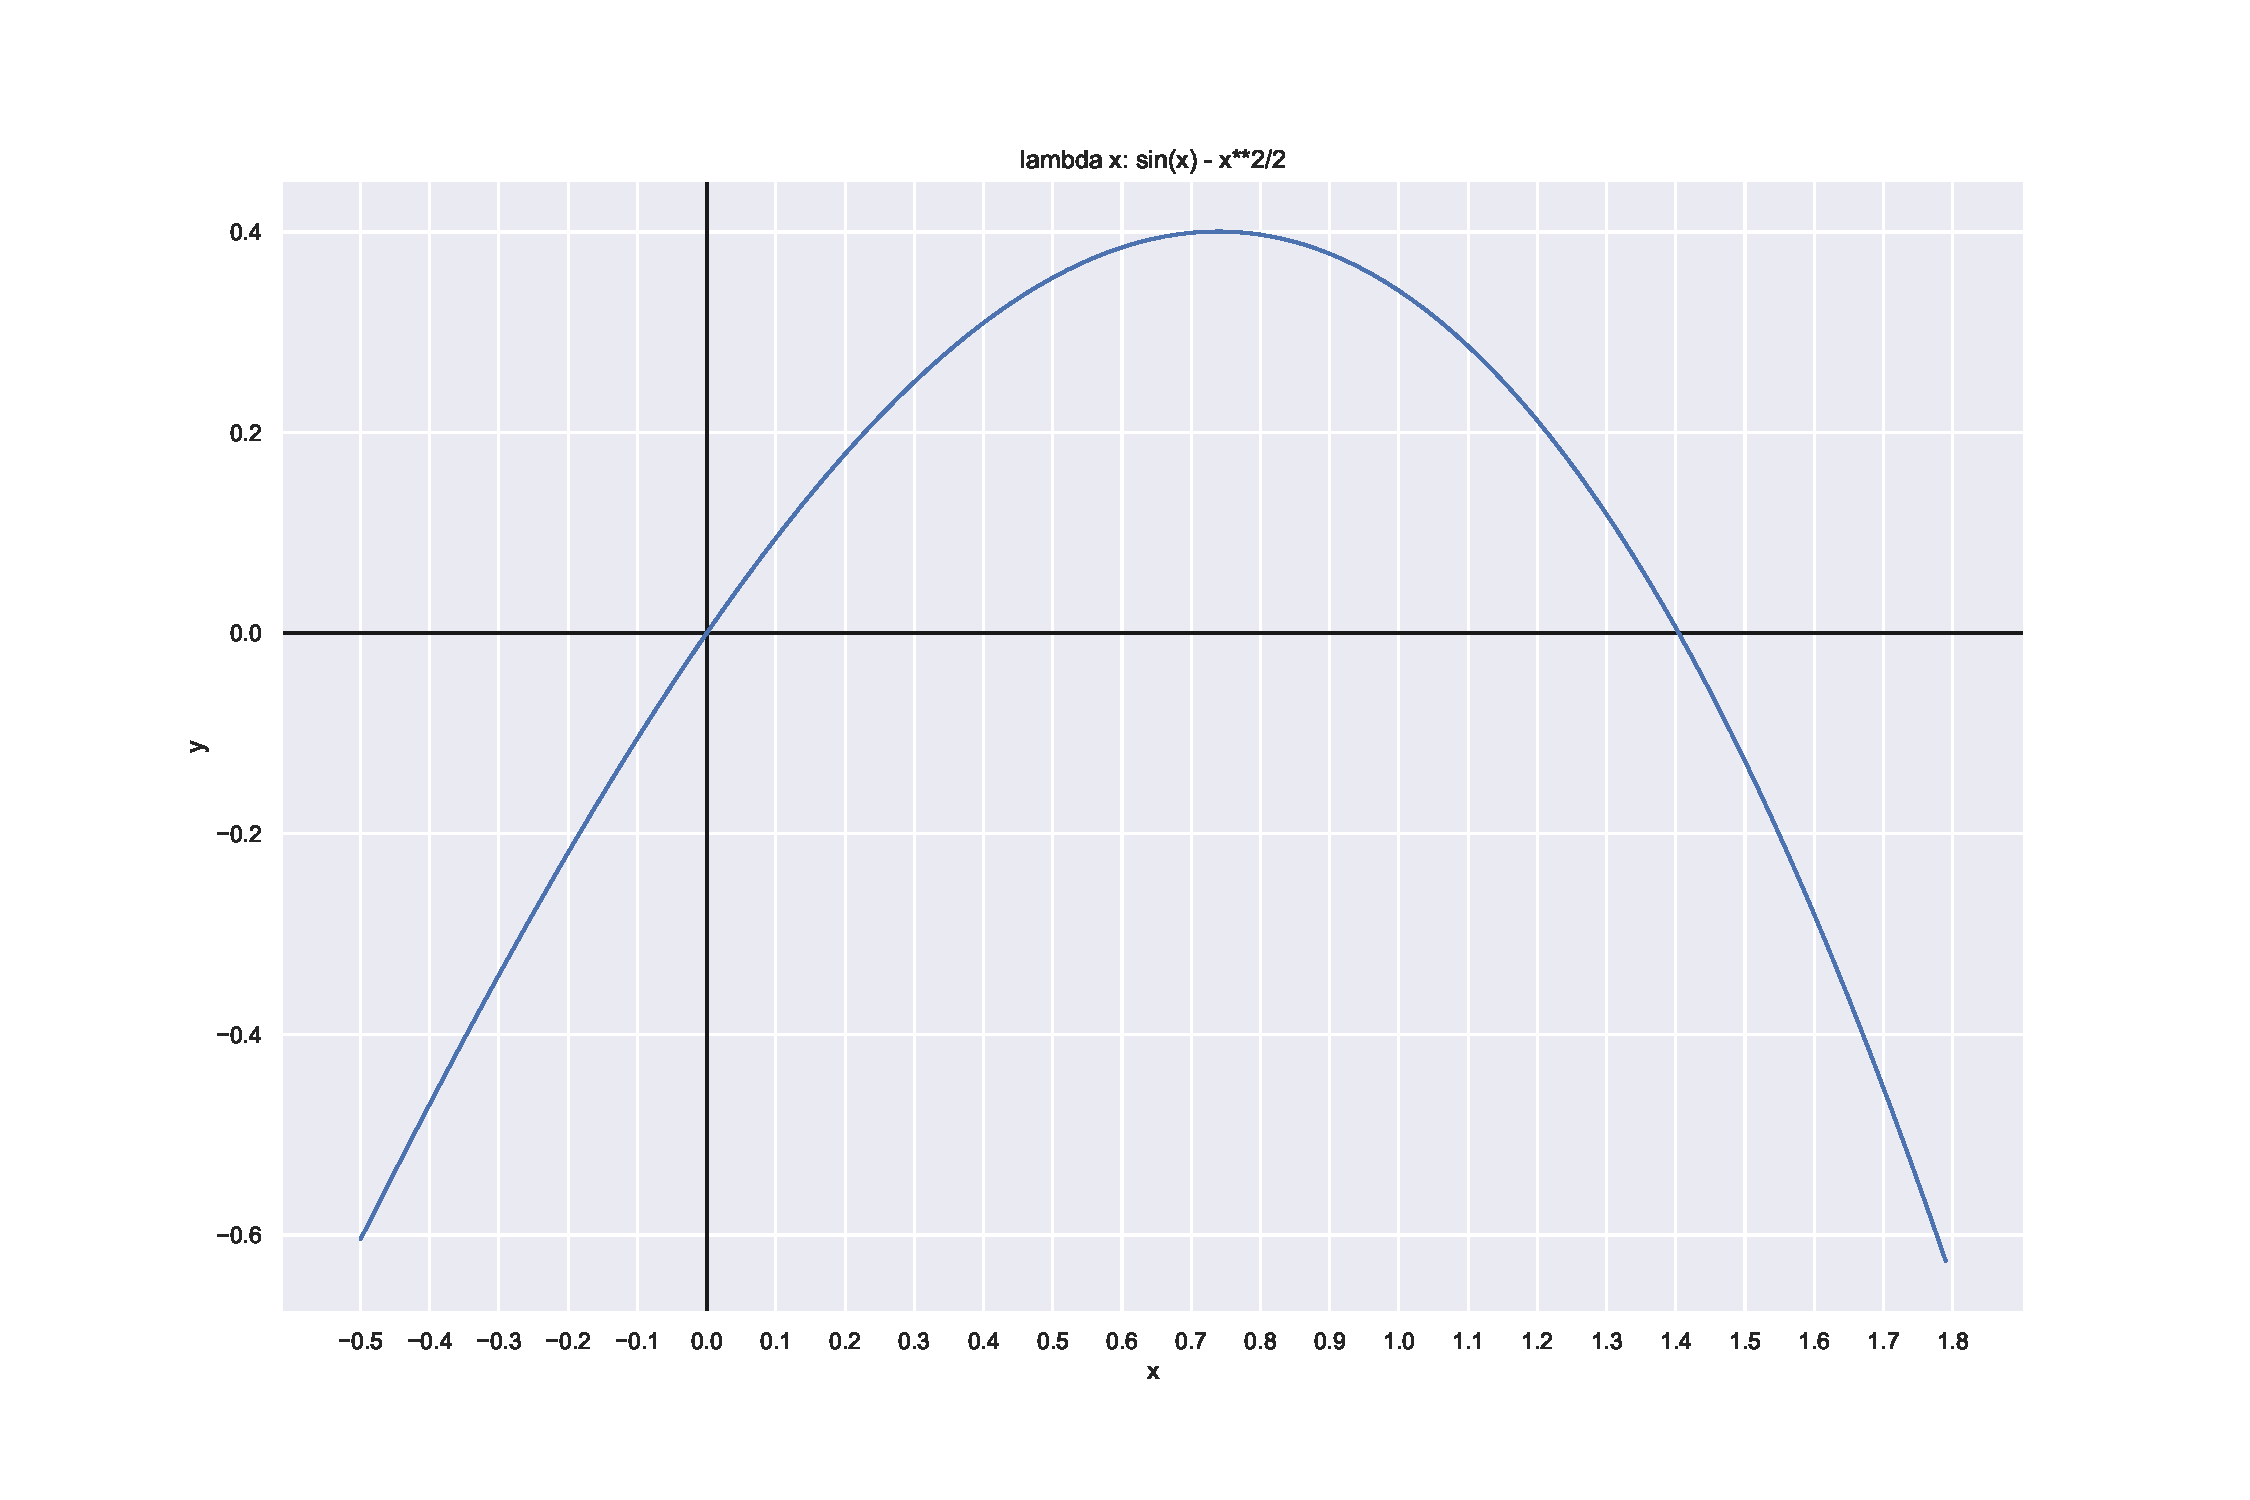
\epsfig{file=Figures/sin-minus-square.pdf, scale=0.5}
\vspace*{-0.3cm}
\caption{The function $x \mapsto \sin(x) - \frac{1}{2} \cdot x^2$.}
\label{fig:sin-minus-square.pdf}
\end{figure}

\noindent
Unfortunately, in many cases the equation 
\\[0.2cm]
\hspace*{1.3cm}
$\nabla f(\mathbf{\widehat{x}}) = \mathbf{0}$
\\[0.2cm]
cannot be solved in \href{https://en.wikipedia.org/wiki/Closed-form_expression}{closed terms}.  This is already
true in the one-dimensional case, i.e.~if $n=1$.  For example, consider 
the function $f:\mathbb{R} \rightarrow \mathbb{R}$ that is defined as
\\[0.2cm]
\hspace*{1.3cm}
$\ds f(x) := \sin(x) - \frac{1}{2} \cdot x^2$.
\\[0.2cm]
This function is shown in Figure \ref{fig:sin-minus-square.pdf} on page \pageref{fig:sin-minus-square.pdf}.
From the graph of the function it is obvious that this function has a maximum somewhere between $0.6$ and
$0.8$.  In order to compute this maximum, we can compute the derivative of $f$.   This derivative is given as 
\\[0.2cm]
\hspace*{1.3cm}
$f'(x) = \cos(x) - x$
\\[0.2cm]
As it happens, the equation $\cos(x) - x = 0$ does not seem to have a solution in 
\href{https://en.wikipedia.org/wiki/Closed-form_expression}{closed form}.  Hence, we can only approximate
the solution numerically via a sequence of numbers $(x_n\bigr)_{n\in\mathbb{N}}$ such that the limit
$\ds \lim\limits_{n\rightarrow\infty} x_n$
exists and is a solution of the equation $\cos(x) - x = 0$, i.e.~we want to have
\\[0.2cm]
\hspace*{1.3cm}
$\ds \cos\Bigl(\lim\limits_{n\rightarrow\infty} x_n\Bigr) = \lim\limits_{n\rightarrow\infty} x_n$.
\\[0.2cm]
The method of \href{https://en.wikipedia.org/wiki/Gradient_descent}{gradient ascent} is a numerical
method that can be used to find the maximum of a function 
\\[0.2cm]
\hspace*{1.3cm}
$f: \mathbb{R}^n \rightarrow \mathbb{R}$
\\[0.2cm]
numerically.  The basic idea is to take a vector $\mathbf{x}_0 \in \mathbb{R}^n$ as the start value and define a sequence of
vectors $\bigl(\mathbf{x}_n\bigr)_{n\in\mathbb{N}}$ such that we have
\\[0.2cm]
\hspace*{1.3cm}
$f(\mathbf{x}_{n+1}) \geq f(\mathbf{x}_{n})$ \quad for all $n\in\mathbb{N}$.
\\[0.2cm]
Hopefully, this sequence will converge against $\widehat{\mathbf{x}} = \arg\max\limits_{\mathbf{x}\in \mathbb{R}^n}f$.
If we do not really know where to start our search, we define $\mathbf{x}_0 := \mathbf{0}$.  In order to
compute $\mathbf{x}_{n+1}$ given $\mathbf{x}_{n}$, the idea is to move from $\mathbf{x}_n$ in that direction
where we have the biggest change in the values of $f$.   This direction happens to be the gradient of $f$ at $\mathbf{x}_n$.
Therefore, the definition of $\mathbf{x}_{n+1}$ is given as follows:
\\[0.2cm]
\hspace*{1.3cm}
$\mathbf{x}_{n+1} := \mathbf{x}_n + \alpha \cdot \nabla f(\mathbf{x}_n)$ \quad for all $n \in \mathbb{N}_0$.
\\[0.2cm]
Here, $\alpha$ is called the \blue{step size} also known as the \blue{learning rate}.  It determines by how
much we move in the direction of the gradient.  In practise, it is best to adapt the step size dynamically
during the iterations.  Figure \ref{fig:gradient-ascent.py} on page \pageref{fig:gradient-ascent.py} shows
how this is done. 
The function \texttt{findMaximum} takes four arguments:
\begin{enumerate}
\item $\texttt{f}$ is the function that is to be maximized.  It is assumed that \texttt{f} takes a vector
      $\texttt{x}\in \mathbb{R}^n$ as its input and that it returns a real number.  Note that $n$ might be
      $1$.  In that case the input to $f$ is a real number.
\item $\texttt{gradF}$ is the gradient of \texttt{f}.  It takes a vector
      $\texttt{x}\in \mathbb{R}^n$ as its input and returns the vector $\nabla \mathtt{f}(\mathtt{x})$.
\item $\texttt{start}$ is a vector from $\mathbb{R}^n$ that is used as the value of $\mathbf{x}_0$.  In
      practice, we will often use $\mathbf{0} \in \mathbb{R}^n$ as the start vector.
\item $\texttt{eps}$ is the precision that we need for the maximum.  We will have to say more on how \texttt{eps}
      is related to the precision later.  As we are using double precision floating point arithmetic, 
      it won't make sense to use a value for \texttt{eps} that is smaller than $10^{-15}$.
\end{enumerate}
Next, let us discuss the implementation of gradient ascent.
\begin{enumerate}
\item \texttt{x} is initialized with the parameter \texttt{start}.  Hence, \texttt{start} is really the same as
      $\mathbf{x}_0$. 
\item \texttt{fx} is the value that the function $f$ takes for the argument \texttt{x}.
\item \texttt{alpha} is the \blue{learning rate}.  We initialize \texttt{alpha} as $1.0$.  The learning rate
      will be adapted dynamically. 
\item The body of the \texttt{while} loop starting in line 6 executes one iteration of gradient ascent.
\item In each iteration, we store the values of $\mathbf{x}_n$ and $f(\mathbf{x}_n)$ in the variables
      \texttt{xOld} and \texttt{fOld}.  This is needed since we need to ensure that the values of
      $f(\mathbf{x}_n)$ are increasing.
\item Next, we compute $\mathbf{x}_{n+1}$ in line 8 using the formula
      \\[0.2cm]
      \hspace*{1.3cm}
      $\mathbf{x}_{n+1} := \mathbf{x}_n + \alpha \cdot \nabla f(\mathbf{x}_n)$.
\item The corresponding value $f(\mathbf{x}_{n+1})$ is computed in line 9.
\item If we are unlucky, $f(\mathbf{x}_{n+1})$ is smaller than $f(\mathbf{x}_{n})$ instead of bigger.  This might happen if the learning
      rate $\alpha$ is too large.  Hence, in this case we decrease the value of $\alpha$, discard 
      both $\mathbf{x}_{n+1}$ and $f(\mathbf{x}_{n+1})$ and start over again via the \texttt{continue}
      statement in line 13.
\item Otherwise, if  $f(\mathbf{x}_{n+1})$ is indeed bigger than $f(\mathbf{x}_{n})$, the vector
  $\mathbf{x}_{n+1}$ is a better approximation of the maximum than the vector $\mathbf{x}_n$.  
      In this case, in order to increase the speed of the convergence of our algorithm we will then increase the learning rate
      $\alpha$ by $20\%$.    
\item The idea of our implementation is to stop the iteration when the relative difference  of 
      $f(\mathbf{x}_{n+1})$ and $f(\mathbf{x}_{n})$ is less than $\varepsilon$ or, to be more precise, if
      \\[0.2cm]
      \hspace*{1.3cm}
      $f(\mathbf{x}_{n+1}) < f(\mathbf{x}_{n}) \cdot (1 + \varepsilon)$.
      \\[0.2cm]
      As the sequence $\bigl(f(\mathbf{x}_n\bigr)_{n\in\mathbb{N}}$ will be monotonically
      increasing, i.e.~we have
      \\[0.2cm]
      \hspace*{1.3cm}
      $f(\mathbf{x}_{n+1}) \geq f(\mathbf{x}_{n})$ \quad for all $n\in\mathbb{N}$,
      \\[0.2cm]
      the condition given above is sufficient.  Now, if the increment of  $f(\mathbf{x}_{n+1})$ is less than $f(\mathbf{x}_{n}) \cdot (1 + \varepsilon)$ 
      we assume that we have reached the maximum with the required precision.  In this case we return both the
      value of \texttt{x} and the corresponding function value $f(\mathtt{x})$.
\end{enumerate}

\begin{figure}[!ht]
\centering
\begin{Verbatim}[ frame         = lines, 
                  framesep      = 0.3cm, 
                  firstnumber   = 1,
                  labelposition = bottomline,
                  numbers       = left,
                  numbersep     = -0.2cm,
                  xleftmargin   = 0.8cm,
                  xrightmargin  = 0.8cm,
                  ]
    def findMaximum(f, gradF, start, eps):
        x     = start
        fx    = f(x)
        alpha = 1.0
        cnt   = 1  # number of iterations
        while True:
            xOld, fOld = x, fx
            x  += alpha * gradF(x)
            fx  = f(x)
            if fx <= fOld:   
                alpha *= 0.5
                x, fx = xOld, fOld
                continue
            else:
                alpha *= 1.2
            if abs(fx - fOld) <= abs(fx) * eps:
                return x, fx
            cnt += 1                  
\end{Verbatim}
\vspace*{-0.3cm}
\caption{The gradient ascent algorithm.}
\label{fig:gradient-ascent.py}
\end{figure}

The implementation of gradient ascent given above is not the most sophisticated variant of this algorithm.
Furthermore, there are algorithms that are more powerful than gradient ascent.  The first of these methods is the
\href{https://en.wikipedia.org/wiki/Conjugate_gradient_method}{conjugate gradient method}.  A
refinement of this method is the
\href{https://en.wikipedia.org/wiki/Broyden-Fletcher-Goldfarb-Shanno_algorithm}{BFGS-algorithm} that
has been invented by Broyden, Fletcher, Goldfarb, and Shanno.  Unfortunately, we do not have the
time to discuss these algorithms.
However, our implementation of gradient ascent is sufficient for our applications and as this is not a course on numerical
analysis but rather on artificial intelligence we will not delve deeper into this topic but, instead, we refer
readers interested in more efficient algorithms to the literature \cite{snyman:2005}.  If you ever need to find
the maximum of a function numerically, you should try to use a predefined library routine that implements a
state of the art algorithm.  For example, in \href{https://www.python.org}{Python} the method
\href{https://docs.scipy.org/doc/scipy/reference/generated/scipy.optimize.minimize.html#scipy.optimize.minimize}{minimize}
from the package \texttt{scipy.optimize} offers various algorithms for minimization.

\section{Logistic Regression}
If we have a model such that 
\\[0.2cm]
\hspace*{1.3cm}
$\mathtt{model}(\mathbf{x}, \mathbf{w}) \approx \mathtt{classify}(\mathbf{x})$
\\[0.2cm]
we want to choose the weight vector $\mathbf{w}$ in a way such that the accuracy 
\\[0.2cm]
\hspace*{1.3cm}
$\ds \mathtt{accuracy}(\mathbf{w}) := 
\frac{\;\cnt \bigl\{ \mathbf{o} \in S \bigm| \mathtt{model}(\mathtt{feature}\bigl(\mathbf{o}),\mathbf{w}\bigr) = \mathtt{classify}(\mathbf{o})\bigr\}\;}{\cnt S}$
\\[0.2cm]
is maximized.  However, there is a snag:  The accuracy is not a smooth function of the weight vector
$\mathbf{w}$.  It can't be a smooth function because the number of errors of our model is a natural number and not a real number
that could change smoothly when the weight vector $\mathbf{w}$ is changed.  Hence, the accuracy is not differentiable as a function
of the weight vector.  The way to proceed is to work with \blue{probabilities} instead.  Instead of assigning a
class to an object $\mathbf{o}$ we rather assign a \blue{probability} $p$ to the object $\mathbf{o}$ that measures how
probable it is that object $\mathbf{o}$ has a given class $c$.  Then we try to maximize this probability.  In
\href{https://en.wikipedia.org/wiki/Logistic_regression}{logistic regression} we use a linear model that is 
combined with the \blue{sigmoid function}.  Before we can discuss the details of logistic regression we need to
define this function and state some of its properties.  

\subsection{The Sigmoid Function}
\begin{Definition}[Sigmoid Function\label{def:sigmoid}]
The \href{https://en.wikipedia.org/wiki/Sigmoid_function}{sigmoid function} $S: \mathbb{R} \rightarrow [0, 1]$ is defined as 
\\[0.2cm]
\hspace*{1.3cm}
$\ds S(t) = \frac{1}{1 + \exp(-t)}$.  
\\[0.2cm]
Figure \ref{fig:sigmoid.eps} on page \pageref{fig:sigmoid.eps} shows the sigmoid function.
\eox
\end{Definition}

\begin{figure}[!ht]
\centering
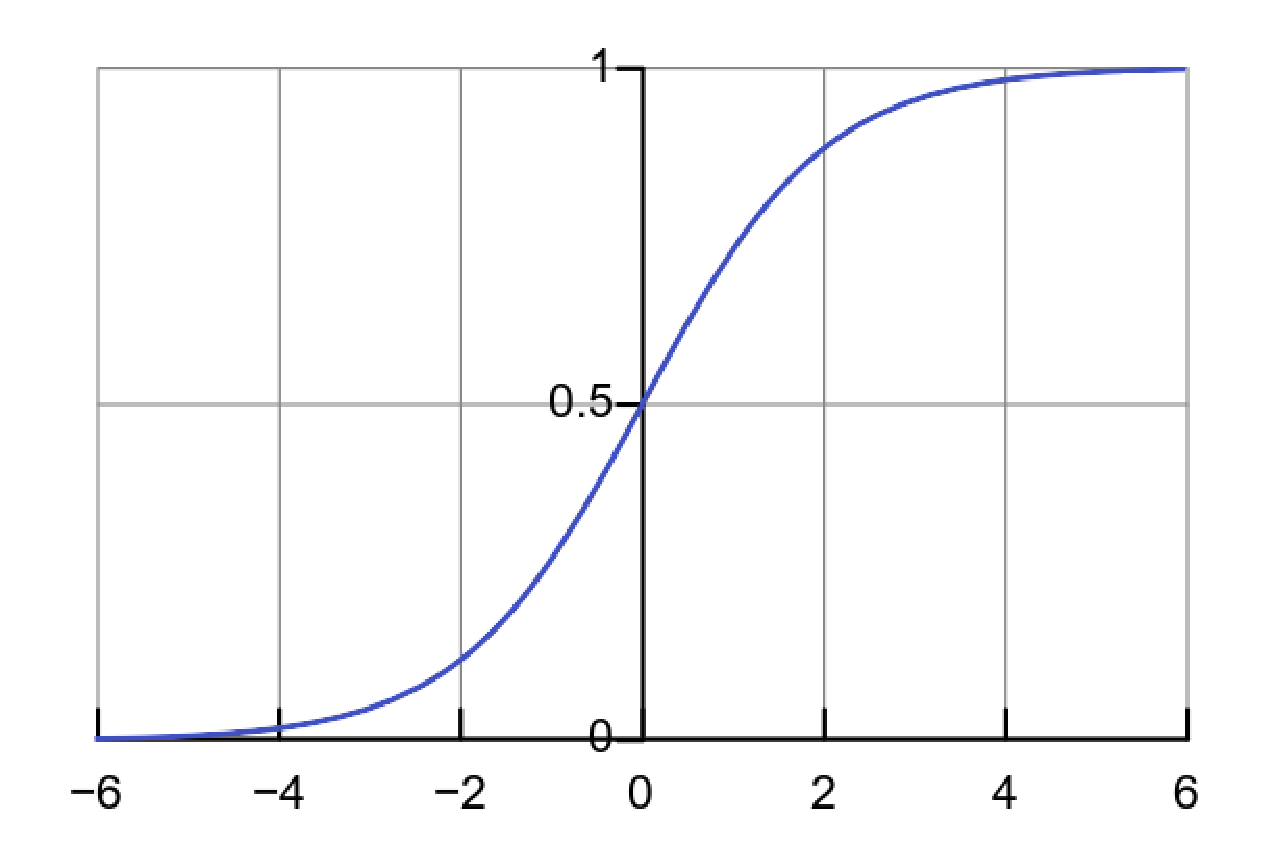
\epsfig{file=Figures/sigmoid.eps, scale=0.7}
\vspace*{-0.3cm}
\caption{The sigmoid function.}
\label{fig:sigmoid.eps}
\end{figure}


\noindent
Let us note some immediate consequences of the definition of the sigmoid function.  As we have
\\[0.2cm]
\hspace*{1.3cm}
$\ds\lim\limits_{x\rightarrow-\infty} \exp(-x) = \infty$, \quad 
$\ds\lim\limits_{x\rightarrow+\infty} \exp(-x) = 0$, \quad and \quad
$\ds\lim\limits_{x\rightarrow\infty} \frac{1}{x} = 0$, 
\\[0.2cm]
the sigmoid function has the following properties:
\\[0.2cm]
\hspace*{1.3cm}
$\ds \lim_{t\rightarrow-\infty} S(t) = 0$ \quad and \quad
$\ds \lim_{t\rightarrow+\infty} S(t) = 1$.
\\[0.2cm]
As the sigmoid function is monotonically increasing, this shows that indeed 
\\[0.2cm]
\hspace*{1.3cm}
$0 \leq S(t) \leq 1$  \quad for all $t \in \mathbb{R}$.
\\[0.2cm]
Therefore, the value of the sigmoid function can be interpreted as a probability.
Another important property of the sigmoid function is its symmetry.  Figure \ref{fig:sigmoid.eps} shows that if the
sigmoid function is shifted down by $\frac{1}{2}$, the resulting function is 
\href{https://en.wikipedia.org/wiki/Point_reflection}{centrally symmetric}, i.e.~we have
\\[0.2cm]
\hspace*{1.3cm}
$\ds S(-t) - \frac{1}{2} = -\Bigl(S(t) - \frac{1}{2}\Bigr)$.
\\[0.2cm]
Adding $\ds\frac{1}{2}$ on both sides of this equation shows that this is equivalent to the equation
\\[0.2cm]
\hspace*{1.3cm}
\colorbox{red}{\framebox{\colorbox{orange}{
$S(-t) = 1 - S(t)$,}}}
\\[0.2cm]
The proof of this fact runs as follows:
\\[0.2cm]
\hspace*{1.3cm}
$
\begin{array}{lcll}
1 - S(t) & = & \ds 1 - \frac{1}{1 + \exp(-t)}             & \mbox{(by definition of $S(t)$)}           \\[0.5cm]
         & = & \ds \frac{1 + \exp(-t) - 1}{1 + \exp(-t)}  & \mbox{(common denominator)}                \\[0.5cm]
         & = & \ds \frac{\exp(-t)}{1 + \exp(-t)}          &                                          \\[0.5cm]
         & = & \ds \frac{1}{\exp(+t) + 1}                 & \mbox{(expand fraction by $\exp(t)$)}      \\[0.5cm]
         & = & \ds \frac{1}{1 + \exp(+t)}                 &                                          \\[0.5cm]
         & = & S(-t)                                      & \mbox{(by definition of $S(-t)$)}. \qquad _\Box
\end{array}
$
\\[0.2cm]
The exponential function can be expressed via the sigmoid function.  Let us start with the definition of the sigmoid
function. 
\\[0.2cm]
\hspace*{1.3cm}
$\ds S(t) = \frac{1}{1 + \exp(-t)}$
\\[0.2cm]
Multiplying this equation with the denominator yields
\\[0.2cm]
\hspace*{1.3cm}
$\ds S(t) \cdot \bigl(1 + \exp(-t)\bigr) = 1$.
\\[0.2cm]
Dividing both sides by $S(t)$ gives:
\\[0.2cm]
\hspace*{1.3cm}
$
\begin{array}{cl}
                & \ds 1 + \exp(-t) = \frac{1}{S(t)}        \\[0.5cm]
\Leftrightarrow & \ds \exp(-t) = \frac{1}{S(t)} - 1        \\[0.5cm]
\Leftrightarrow & \ds \exp(-t) = \frac{1 - S(t)}{S(t)}      
\end{array}
$
\\[0.2cm]
We highlight this formula, as we need it later
\begin{equation}
\label{eq:1}
 \colorbox{red}{\framebox{\colorbox{orange}{\mbox{$\ds\exp(-t) = \frac{1 - S(t)}{S(t)}$.}}}}
\end{equation}
If we take the reciprocal of both sides of this equation, we have
\\[0.2cm]
\hspace*{1.3cm}
$\ds \exp(t) = \frac{S(t)}{1 - S(t)}$.
\\[0.2cm]
Applying the natural logarithm on both sides of this equation yields
\\[0.2cm]
\hspace*{1.3cm}
$\ds t = \ln\left(\frac{S(t)}{1-S(t)}\right)$.
\\[0.2cm]
This shows that the inverse of the sigmoid function is given as
\\[0.2cm]
\hspace*{1.3cm}
\colorbox{red}{\framebox{\colorbox{orange}{
$\ds S^{-1} (y) = \ln\left(\frac{y}{1-y}\right)$.}}} 
\\[0.2cm]
This function is known as the \href{https://en.wikipedia.org/wiki/Logit}{logit function}.
Next, let us compute the derivative of $S(t)$, i.e.~$\ds S'(t) =\frac{\mathrm{d}S}{\mathtt{d}t}$.  We have
\\[0.2cm]
\hspace*{1.3cm}
$
\begin{array}{lcll}
 S'(t) & = & \ds -\frac{-\exp(-t)}{\bigr(1+\exp(-t)\bigr)^2}   \\[0.5cm]
       & = & \ds \exp(-t) \cdot S(t)^2                         \\[0.2cm]
       & = & \ds \frac{1-S(t)}{S(t)} \cdot S(t)^2  & \mbox{(by Equation \ref{eq:1})} \\[0.4cm]
       & = & \ds \bigl(1 - S(t)\bigr) \cdot S(t)            
\end{array}
$
\\[0.2cm]
We have shown
\begin{equation}
  \label{eq:2}
  \colorbox{red}{\framebox{\colorbox{orange}{\mbox{$\ds S'(t) = \bigl(1 - S(t)\bigr) \cdot S(t)$.}}}}
\end{equation}
We will later need the derivative of the natural logarithm of the logistic function.  We define
\\[0.2cm]
\hspace*{1.3cm}
$L(t) := \ln\bigl(S(t)\bigr)$.
\\[0.2cm]
Then we have
\\[0.2cm]
\hspace*{1.3cm}
$
\begin{array}{lcll}
  L'(t) & = & \ds \frac{S'(t)}{S(t)}                  & \mbox{(by the chain rule)} \\[0.5cm]
        & = & \ds \frac{(1 - S(t)) \cdot S(t)}{S(t)}                               \\[0.5cm]
        & = & \ds 1 - S(t)                                                         \\[0.2cm]
        & = & \ds S(-t)                               & \mbox{(by symmetry)} 
\end{array}
$
\\[0.2cm]
% If we have the function $f(t) := L(-t)$, then we see that
%\\[0.2cm]
%\hspace*{1.3cm}
% $f'(t) = -S(t)$
%\\[0.2cm]
% holds.   
As this is our most important result, we highlight it:
\\[0.2cm]
\hspace*{1.3cm}
\colorbox{red}{\framebox{\colorbox{orange}{$L'(t) = S(-t)$ \quad where \quad $L(t) := \ln\bigl(S(t)\bigr)$.}}}


\subsection{The Model of Logistic Regression}
In logistic regression we deal with \blue{binary classification}, i.e.~we assume that we just need to decide
whether a given object is a member of a given class or not.  We use the following model to compute the \blue{probability} that an
object $o$ with features $\mathbf{x}$ will be of the given class: 
\\[0.2cm]
\hspace*{1.3cm}
$P(y=+1\;|\;\mathbf{x},\mathbf{w}) = S(\mathbf{x} \cdot \mathbf{w})$.
\\[0.2cm]
Note that $P(y=+1\;|\;\mathbf{x},\mathbf{w})$ is the \blue{conditional probability} that $o$ has the given
class, given its features $\mathbf{x}$ and the weights $\mathbf{w}$.  The expression $\mathbf{x}
\cdot \mathbf{w}$ denotes the \blue{dot product} of the vectors $\mathbf{x}$ and $\mathbf{w}$,  
i.e. we have
\\[0.2cm]
\hspace*{1.3cm}
$\mathbf{x} \cdot \mathbf{w} = \sum\limits_{i=1}^D x_i \cdot w_i$.
\\[0.2cm] 
To simplify calculations, it is assumed that $\mathbf{x}$ contains a \blue{constant feature} that always takes the value of $1$.
Seeing this model the first time you might think that this model is not very general and that it can only be
applied in very special circumstances.  However, the fact is that the features $x_i$ can be functions of arbitrary complexity
and hence this model is much more general than it appears on first sight.

We assume that $y$ can only take the values $+1$ or $-1$,  e.g.~in the example of spam detection $y = 1$ if the
email is spam and $y = -1$ otherwise.  Since complementary probabilities add up to $1$, we have
\\[0.2cm]
\hspace*{1.3cm}
$P(y=-1\;|\;\mathbf{x},\mathbf{w}) = 1 - P(y=+1\;|\;\mathbf{x},\mathbf{w}) 
  = 1 - S(\mathbf{x} \cdot \mathbf{w}) = S(-\mathbf{x} \cdot \mathbf{w})
$.
\\[0.2cm]
Hence, we can combine the equations for $P(y=-1\;|\;\mathbf{x},\mathbf{w})$ and $P(y=+1\;|\;\mathbf{x},\mathbf{w})$ into a
single equation
\\[0.2cm]
\hspace*{1.3cm}
\colorbox{red}{\framebox{\colorbox{orange}{$P(y\;|\;\mathbf{x},\mathbf{w}) = S\bigl(y \cdot(\mathbf{x} \cdot \mathbf{w})\bigr)$.}}}
\\[0.2cm]
Given $N$ objects $o_1, \cdots, o_n $ with feature vectors $\mathbf{x}_1, \cdots, \mathbf{x}_n$ and classes
$y_1,\cdots,y_n$, we
want to determine the weight vector $\mathbf{w}$ such that the \blue{likelihood} $\ell(\mathbf{X}, \mathbf{y})$ of all of our
observations is maximized.  This approach is called the 
\href{https://en.wikipedia.org/wiki/Maximum_likelihood_estimation}{maximum likelihood estimation} of the weights.
As we assume that the probabilities of different observations are independent, the individual
probabilities have to be multiplied to compute the overall likelihood $\ell(\mathbf{X}, \mathbf{y},\mathbf{w})$ 
of a given training set:
\\[0.2cm]
\hspace*{1.3cm}
$\ds \ell(\mathbf{X},\mathbf{y},\mathbf{w}) = \prod\limits_{i=1}^N P(y_i \;|\;\mathbf{x}_i,\mathbf{w})$.
\\[0.2cm]
Here, we have combined the different attribute vectors $\mathbf{x}_i$ into the matrix $\mathbf{X}$ such that
$\mathbf{x}_i$ is the $i$-th row of the matrix $\mathbf{X}$.  Since it is
easier to work with sums than with products, instead of maximizing the function
$\ell(\mathbf{X},\mathbf{y},\mathbf{w})$ we instead maximize the logarithm of
$\ell(\mathbf{X},\mathbf{y},\mathbf{w})$.  This logarithm is called the \blue{log-likelihood} and is defined as 
\\[0.2cm]
\hspace*{1.3cm}
$\ell\ell(\mathbf{X},\mathbf{y},\mathbf{w}) := \ln\bigl(\ell(\mathbf{X},\mathbf{y},\mathbf{w})\bigr)$. 
\\[0.2cm]
As the natural logarithm is a \href{https://en.wikipedia.org/wiki/Monotonic_function}{monotonically increasing}
function, the functions $\ell(\mathbf{X},\mathbf{y},\mathbf{w})$ and  $\ell\ell(\mathbf{X},\mathbf{y},\mathbf{w})$ take their maximum at the same value of $\mathbf{w}$.  As we have
\\[0.2cm]
\hspace*{1.3cm}
$\ln(a \cdot b) = \ln(a) + \ln(b)$,
\\[0.2cm]
the natural logarithm of the likelihood is 
\\[0.2cm]
\hspace*{1.3cm}
\colorbox{red}{\framebox{\colorbox{orange}{
$\ds \ell\ell(\mathbf{X},\mathbf{y},\mathbf{w}) = 
 \sum\limits_{i=1}^N \ln\Bigl(S\bigl(y_i \cdot(\mathbf{x}_i \cdot \mathbf{w})\bigr)\Bigr) =
 \sum\limits_{i=1}^N L\bigl(y_i \cdot(\mathbf{x}_i \cdot \mathbf{w})\bigr)
$.}}}
\\[0.2cm]
Our goal is to choose the weights $\mathbf{w}$ such that the likelihood is maximized.  Since this is the same as maximizing the log-likelihood, we
need to determine those values of the coefficients $\mathbf{w}$ that satisfy
\\[0.2cm]
\hspace*{1.3cm}
$\ds \frac{\partial\quad}{\partial\, w_j}\ell\ell(\mathbf{X},\mathbf{y},\mathbf{w}) = 0$.
\\[0.2cm]
In order to compute the partial derivative of $\ell\ell(\mathbf{X},\mathbf{y},\mathbf{w})$ with respect to the
coefficients $\mathbf{w}$ we need to compute the partial derivative of the dot product $\mathbf{x}_i \cdot
\mathbf{w}$ with respect to the weights $w_j$.
We define
\\[0.2cm]
\hspace*{1.3cm}
$\ds h(\mathbf{w}) := \mathbf{x}_i \cdot \mathbf{w} = \sum\limits_{k=1}^D x_{i,k} \cdot w_k$.
\\[0.2cm]
Then we have
\\[0.2cm]
\hspace*{1.3cm}
$\ds \frac{\partial\quad}{\partial\, w_j} h(\mathbf{w})
   = \frac{\partial\quad}{\partial\, w_j} \sum\limits_{k=1}^D x_{i,k} \cdot w_k
   = \sum\limits_{k=1}^D x_{i,k} \cdot \frac{\partial\quad}{\partial\, w_j} w_k
   = \sum\limits_{k=1}^D x_{i,k} \cdot \delta_{j,k} =  x_{i,j}
$.
\\[0.2cm]
Now we are ready to compute the partial derivative of $\ell\ell(\mathbf{X},\mathbf{y},\mathbf{w})$ with respect to $\mathbf{w}$:
\\[0.2cm]
\hspace*{1.3cm}
$
\begin{array}{cll}
  & \ds \frac{\partial\quad}{\partial\, w_j} \ell\ell(\mathbf{X},\mathbf{y},\mathbf{w}) \\[0.5cm]
= & \ds \frac{\partial\quad}{\partial\, w_j} 
    \sum\limits_{i=1}^N L\bigl(y_i \cdot(\mathbf{x}_i \cdot \mathbf{w})\bigr) 
    \\[0.5cm]
= & \ds\sum\limits_{i=1}^N y_i \cdot x_{i,j} \cdot  S\bigl(-y_i \cdot(\mathbf{x}_i \cdot \mathbf{w})\bigr),
  & \mbox{since} \quad \ds \frac{\mathrm{d}L(x)}{\mathrm{d}x} = S(-x).
\end{array}
$
\\[0.2cm]
Hence, the partial derivative of the log-likelihood function is given as follows:
\\[0.2cm]
\hspace*{1.3cm}
\colorbox{red}{\framebox{\colorbox{orange}{
$\ds \frac{\partial\quad}{\partial\, w_j}\ell\ell(\mathbf{X},\mathbf{y},\mathbf{w}) =
 \ds\sum\limits_{i=1}^N y_i \cdot x_{i,j} \cdot  S(-y_i \cdot \mathbf{x}_i \cdot \mathbf{w})
$}}} 
\\[0.2cm]
Next, we have to find the value of $\mathbf{w}$ such that
\\[0.2cm]
\hspace*{1.3cm}
$\ds\sum\limits_{i=1}^N y_i \cdot x_{i,j} \cdot  S(-y_i \cdot \mathbf{x}_i \cdot \mathbf{w}) = 0$
\quad for all $j \in \{1, \cdots, D\}$.
\\[0.2cm]
These are $D$ equations for the $D$ variables $w_1, \cdots, w_D$.  Due to the occurrence of the sigmoid function, these
equations are nonlinear.  We can not solve these equations explicitly.  Nevertheless, our computation of the
gradient of the log-likelihood was not for in vain:  We will use the method of gradient ascent in order to find
the value of $\mathbf{w}$ that maximizes the log-likelihood.  This method has been outlined in the previous section.

\subsection{Implementing Logistic Regression}

In this section we will give a simple implementation of logistic regression.  We will use our implementation of
logistic regression to predict whether a student will pass or fail a given exam.  Figure \ref{fig:exam.csv}
shows a \href{https://en.wikipedia.org/wiki/Comma-separated_values}{\textsc{Csv}} file that contains the data
we are going to explore.  Concretely, this file stores the hours a student has learned for a particular exam
and the fact whether the student has passed the exam or has failed.  A passed exam is encoded as the number
$1$, while a failed exam is encoded as $0$.  The first column of the file stores these numbers.  The second
column stores the number of hours that the student has learned in order to pass the exam.


\begin{figure}[!ht]
\centering
\begin{Verbatim}[ frame         = lines, 
                  framesep      = 0.3cm, 
                  firstnumber   = 1,
                  labelposition = bottomline,
                  numbers       = left,
                  numbersep     = -0.2cm,
                  xleftmargin   = 0.8cm,
                  xrightmargin  = 0.8cm,
                ]
   Pass, Hours
   0,    0.50
   0,    0.75
   0,    1.00
   0,    1.25
   0,    1.50
   0,    1.75
   1,    1.75
   0,    2.00
   1,    2.25
   0,    2.50
   1,    2.75
   0,    3.00
   1,    3.25
   0,    3.50
   1,    4.00
   1,    4.25
   1,    4.50
   1,    4.75
   1,    5.00
   1,    5.50
\end{Verbatim}
\vspace*{-0.3cm}
\caption{Results of an exam.}
\label{fig:exam.csv}
\end{figure}

The program shown in Figure \ref{fig:logistic_regression.py} on page
\pageref{fig:logistic_regression.py} implements logistic regression.  As there are a number of
subtle points that might easily be overlooked otherwise, we proceed to discuss this program line by line. 


\begin{figure}[!ht]
\centering
\begin{Verbatim}[ frame         = lines, 
                  framesep      = 0.3cm, 
                  firstnumber   = 1,
                  labelposition = bottomline,
                  numbers       = left,
                  numbersep     = -0.2cm,
                  xleftmargin   = 0.8cm,
                  xrightmargin  = 0.8cm,
                ]
    import numpy as np
    
    def sigmoid(t):
        "compute the sigmoid of t"
        return 1.0 / (1.0 + np.exp(-t))
    
    def logSigmoid(t):
        "compute the sigmoid of t, avoid overflow"
        if t > -100:
            return -np.log(1.0 + np.exp(-t))
        else:
            return t
    
    def ll(X, y, w):
        """
        given the matrix X and the observations y,
        return the log likelihood for the weight vector w
        """
        return np.sum([logSigmoid(y[i] * (X[i] @ w)) for i in range(len(X))])
    
    def gradLL(X, y, w):
        """
        Compute the gradient ofthe log-likelihood with respect to w 
        """
        Gradient = []
        for j in range(len(X[1])):
            L = [y[i]*X[i][j]*sigmoid(-y[i] * (X[i] @ w)) for i in range(len(X))]
            Gradient.append(sum(L))
        return np.array(Gradient)
\end{Verbatim}
\vspace*{-0.3cm}
\caption{An implementation of logistic regression.}
\label{fig:logistic_regression.py}
\end{figure}



\begin{enumerate}
\item First, we \texttt{import} the module \texttt{numpy}.  This module provides us with the 
      functions \texttt{log} and \texttt{exp} for computing the logarithm and the exponential of a number or
      vector.  Furthermore, we need this module because the gradient of the log-likelihood is a vector and for
      efficiency reasons this vector should be stored as a NumPy array.
\item Line 3 implements the sigmoid function

      \hspace*{1.3cm}
      $\ds S(x) = \frac{1}{1 + \exp(-x)}$.
      \\[0.2cm]
      Since we are using NumPy to compute the exponential function, the parameter $t$ that is used in our
      implementation can also be a vector.
\item Line 7 starts the implementation of the natural logarithm of the sigmoid function, i.e.~we implement
      \\[0.2cm]
      \hspace*{1.3cm}
      $\ds L(x) = \ln\bigl(S(X)\bigr) = \ln\left(\frac{1}{1 + \exp(-x)}\right) =- \ln\bigl(1 + \exp(-x)\bigr)$.
      \\[0.2cm]
      The implementation is more complicated than you might expect.  The reason has to do with
      overflow.  Consider values of $x$ that are smaller than, say, $-1000$.  The problem is that
      the expression $\mathtt{exp}(1000))$ evaluates to \texttt{Infinity}, which represents the
      mathematical value $\infty$.  But then $1 + \mathtt{exp}(1000))$ is also \texttt{Infinity} and
      finally \texttt{log(1 + exp(1000))} is \texttt{Infinity}.  However, in reality we have
      \\[0.2cm]
      \hspace*{1.3cm}
      $\ln\bigl(1 + \exp(1000)\bigr) \approx 1000$
      \\[0.2cm] 
      because $\exp(1000)$ is so big that adding $1$ to it does not make much of a difference.
      The precise argument works as follows:
      \\[0.2cm]
      \hspace*{1.3cm}
      $
      \begin{array}{lcll}
        \ln\bigl(1+\exp(x)\bigr) & = & \ln\bigl(\exp(x) \cdot (1+\exp(-x))\bigr)          \\[0.2cm]
                                 & = & \ln\bigl(\exp(x)\bigr) + \ln\bigl(1+\exp(-x)\bigr) \\[0.2cm]
                                 & = & x + \ln\bigl(1+\exp(-x)\bigr) \\[0.2cm]
                                 & \approx & x + \ln(1) + \exp(-x) & \mbox{Taylor expansion of $\ln(1+x)$} \\[0.2cm]
                                 & = & x + 0 + \exp(-x)                                      \\[0.2cm]
                                 & \approx & x                & \mbox{since $\exp(-x) \approx 0$ for large $x$} 
      \end{array}
      $
      \\[0.2cm]
      This is the reason that \texttt{logSigmoid} returns \texttt{x} if the value of \texttt{x} is less than
      $-100$.
\item The function $\mathtt{ll}(\mathbf{X}, \mathbf{y}, \mathbf{w})$ defined in line 14 computes the
      log-lokelihood of the parameter $\mathbf{w}$ given the available data $\mathbf{X}$ and $\mathbf{y}$.
      We have
      \\[0.2cm]
      \hspace*{1.3cm}
      $\ds \ell\ell(\mathbf{X},\mathbf{y};\mathbf{w}) = 
           \sum\limits_{i=1}^N L\bigl(y_i \cdot(\mathbf{x}_i \cdot \mathbf{w})\bigr)
      $.
      \\[0.2cm]
      Here $L$ denotes the natural logarithm of the sigmoid of the argument.
      It is assumed that $\mathbf{X}$ is a matrix.  Every observation corresponds to a row in this
      matrix, i.e.~the vector $\mathbf{x}_i$ is the feature vector containing the features of the
      $i$-th observation.  $\mathbf{y}$ is a vector describing the outcomes, i.e.~the elements
      of this vector are either $+1$ or $-1$.  Finally, $\mathbf{w}$ is the vector of coefficients.
\item The function $\mathtt{gradLL}(\mathbf{x}, \mathbf{y}, \mathbf{w})$ in line 21 computes the gradient of
      the log-lokelihood according to the formula
      \\[0.2cm]
      \hspace*{1.3cm}
      $\ds \frac{\partial\quad}{\partial\, w_j}\ell\ell(\mathbf{X},\mathbf{y};\mathbf{w}) =
        \ds\sum\limits_{i=1}^N y_i \cdot x_{i,j} \cdot  S(-y_i \cdot \mathbf{x}_i \cdot \mathbf{w})
      $.
      \\[0.2cm]
      The different components of this gradient are combined into a vector.
      The arguments are the same as the arguments to the log-lokelihood.
\item Finally, the function \texttt{logisticRegressionFile} that is shown in Figure
      \ref{fig:logistic_regression.py:2} takes one argument.  This argument
      is the name of the \texttt{.csv} file containing the data that are to be analysed.  
      The task of this function is to read the \textsc{Csv} file, convert the data in the feature matrix
      $\mathbf{X}$ and the vector $\mathbf{y}$, and then to use the method of gradient ascent to find the weight vector
      $\mathbf{w}$ that maximize the likelihood.  In detail this function works as follows.
      \begin{enumerate}
      \item The \texttt{with} statement that extends from line 34 to line 43 reads the data in the file that
            is specified by the parameter \texttt{name}.
      \item After the data has been read, the list \texttt{Pass} contains a list of floating point numbers that
            are either $0$ or $1$ specifying whether the student has passed the exam, while the list
            \texttt{Hours} contains the numbers of hours that the students have spend studying.
      \item These data are converted into the NumPy arrays \texttt{x} and \texttt{y} in line 44 and 45.
      \item \texttt{n} is the number of data points we have, i.e.~it is the number of students.
      \item We reshape the vector \texttt{x} into a matrix \texttt{X} in line 47.
            As there is only a single feature, namely the hours a student has studied, all rows of this matrix
            have a length of $1$. 
      \item Next, we prepend a column of ones to this matrix.  This is done in line 48.
      \item In logistic regression we assume that the entries of the vector $\mathbf{y}$ are either $+1$ or
            $-1$.  As the data provided in our input file contains $1$ and $0$, we need to apply a function that maps $1$ to $+1$ and $0$ to $-1$.
            The function
            \\[0.2cm]
            \hspace*{1.3cm}
            $y \mapsto 2 \cdot y - 1$
            \\[0.2cm]
            fits this job description and is applied to transform the vector $\mathbf{y}$ appropriately in line
            49.
      \item Now we are ready to run gradient ascent.  As the start vector we use a vector containing only
            zeros.  This vector is defined in line 50.  The precision we use is $10^{-8}$.
            We want to maximize the log-lokelihood of a given weight vector $\mathtt{w}$.  Hence we define the
            function $\texttt{f}(\texttt{w})$ as $\mathtt{ll}(\mathtt{X}, \mathtt{y}, \mathtt{w})$ in line 52,
            while the gradient of this function is defined in line 53.
            Line 54 call the function \texttt{gradient\_ascent} that computes the value of \texttt{w} that
            maximizes the log-lokelihood.            
      \end{enumerate}
\end{enumerate}

\begin{figure}[!ht]
\centering
\begin{Verbatim}[ frame         = lines, 
                  framesep      = 0.3cm, 
                  firstnumber   = last,
                  labelposition = bottomline,
                  numbers       = left,
                  numbersep     = -0.2cm,
                  xleftmargin   = 0.8cm,
                  xrightmargin  = 0.8cm,
                ]
    import csv
    import gradient_ascent

    def logisticRegression(name):
        with open(name) as file:
            reader = csv.reader(file, delimiter=',')
            count  = 0  # line count
            Pass   = []
            Hours  = []
            for row in reader:
                if count != 0:  # skip header
                    Pass .append(float(row[0]))
                    Hours.append(float(row[1]))
                count += 1
        y = np.array(Pass)
        x = np.array(Hours)
        n = len(y)
        X = np.reshape(x, (n,1))
        X = np.append(np.ones((n, 1)), X, axis=-1)
        y = 2 * y - 1
        start   = np.zeros((2,))
        eps     = 10 ** -8
        f       = lambda w: ll(X, y, w)
        gradF   = lambda w: gradLL(X, y, w)
        w, _, _ = gradient_ascent.findMaximum(f, gradF, start, eps)
        return w
\end{Verbatim}
\vspace*{-0.3cm}
\caption{The function \texttt{logisticRegression}.}
\label{fig:logistic_regression.py:2}
\end{figure}

If we run the function \texttt{logisticRegressionFile} using the data shown in Figure
\ref{fig:exam.csv} the resulting values of the weight vector \texttt{w} are
\\[0.2cm]
\hspace*{1.3cm}
\texttt{[-4.0746468959343405, 1.5033787070592017]}
\\[0.2cm]
This shows that the probability $P(h)$ that a student who has studied for $h$ hours will pass the
exam is given approximately as follows:
\\[0.2cm]
\hspace*{1.3cm}
$\ds P(h) \approx \frac{1}{1 + \exp(4.1 - 1.5 \cdot h)}$
\\[0.2cm]
Figure \ref{fig:exam-probability.pdf} shows a plot of this probability $P(x)$.  

\begin{figure}[!th]
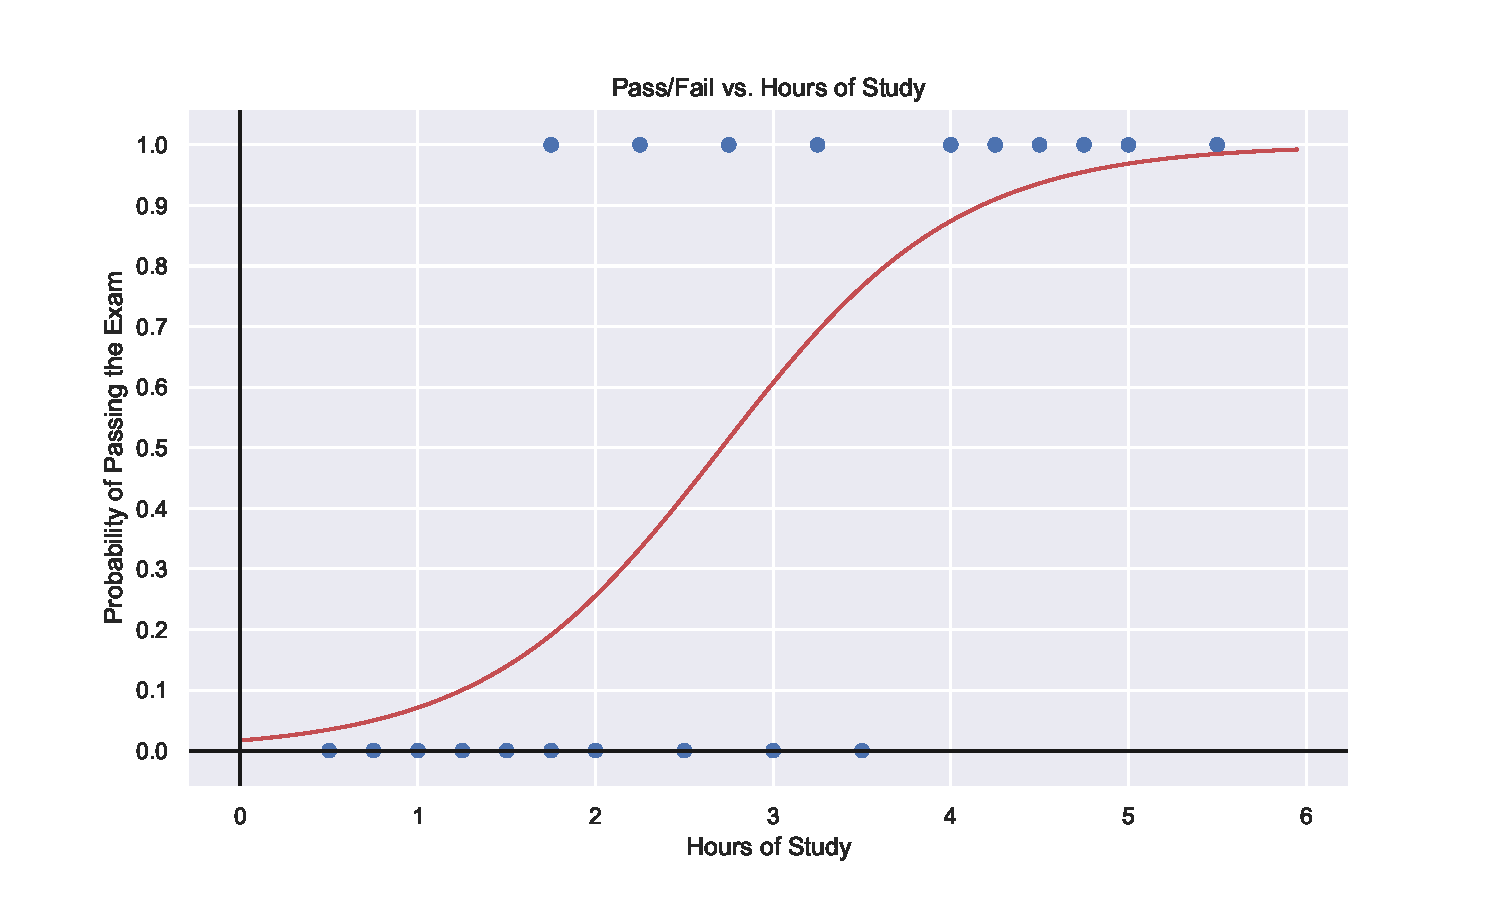
\epsfig{file=Figures/exam-probability.pdf, scale=0.7}
\caption{Probability of passing an exam versus hours of studying.}
\label{fig:exam-probability.pdf}
\end{figure}


\exercise 
The file \href{https://github.com/karlstroetmann/Artificial-Intelligence/blob/master/Python/iris.csv}{iris.csv}
contains the sizes of both the \href{https://en.wikipedia.org/wiki/Sepal}{sepals} and the
\href{https://en.wikipedia.org/wiki/Pepal}{petals} of three different specimen of the iris flower.  The
data is described in more detail \href{https://en.wikipedia.org/wiki/Iris_flower_data_set}{here}. 
Use logistic regression to predict whether a given plant is of the species
\href{https://en.wikipedia.org/wiki/Iris_setosa}{iris setosa} (Deutsch: Borsten-Schwertlilie),
\href{https://en.wikipedia.org/wiki/Iris_virginica}{iris virginica}\footnote{
This plant is native to North America and hence has no German name.}, or
\href{https://en.wikipedia.org/wiki/Iris_versicolor}{iris versicolor} (Deutsch: Verschiedenfarbige Schwertlilie).
As logistic regression is only able to distinguish between two different classes, you
have to build three different classifiers:
\begin{itemize}
\item The first classifier is able to distinguish \blue{iris setosa} from other irises. 
\item The second classifier is able to distinguish \blue{iris virginica} from other irises. 
\item The third classifier is able to distinguish \blue{iris versicolor} from other irises. 
\end{itemize}
Your task is to implement these classifiers and to evaluate their accuracy.  
You should  divide the data randomly into a \blue{training dataset}, which is used for computing the
coefficients of logistic regression and a \blue{test dataset}, which you should only use to predict the
accuracy of your model.  To this end, the function
\\[0.2cm]
\hspace*{1.3cm}
\texttt{sklearn.model\_selection.train\_test\_split}
\\[0.2cm]
might be useful.  Once you have created these classifiers, proceed to implement a classifier that inputs a
feature vector and that outputs the class of the iris flower as a string.  If you do this correctly, you can
achieve an accuracy of $100\%$.
\eox

\section{Naive Bayes Classifiers}
In this section we discuss \href{https://en.wikipedia.org/wiki/Naive_Bayes_classifier}{naive Bayes classifiers}.
Naive Bayes classifiers are an alternative method for classification which is appropriate in cases where the
features are not numerical but categorical.  It starts with \href{https://en.wikipedia.org/wiki/Bayes%27_theorem}{Bayes' theorem}:
Assume we have some evidence $E$ about an object $o$ and want to know whether $o$ belongs to some class $C$.
Bayes' theorem tell us that the conditional probability $P(C|E)$, i.e the probability that $o$ has class $C$
given that we have observed the evidence $E$, is related to the conditional probability $P(E|C)$, which is the probability that we
observe the evidence $E$ given that $o$ has class $C$, in the following way:
\\[0.2cm]
\hspace*{1.3cm}
$\ds P(C|E) = \frac{P(E|C) \cdot P(C)}{P(E)}$.
\\[0.2cm]
This theorem is useful because often the conditional probability $P(E|C)$ that we observe some evidence $E$ in an object
$o$ of class $C$ is readily available, but the conditional probability $P(C|E)$ that an object has class $C$ if
we have observed the evidence $E$ is unknown.  In the context of machine learning the evidence $E$ is often
given as a list of features $f_1$, $\cdots$, $f_m$ that we are able to observe or compute.  In this case we
have to rewrite Bayes' theorem as follows:
\\[0.2cm]
\hspace*{1.3cm}
$\ds P(C\;|\;f_1 \wedge \cdots \wedge f_m) = \frac{P(f_1 \wedge \cdots \wedge f_m\;|\;C) \cdot P(C)}{P(f_1 \wedge \cdots \wedge f_m)}$.
\\[0.2cm]
In order to apply this form of Bayes' theorem to the problem of classification, we have to rewrite the expression
\\[0.2cm]
\hspace*{1.3cm}
$P(f_1 \wedge \cdots \wedge f_m\;|\;C)$.
\\[0.2cm]
The conditional probability $P(A|B)$ that an event $A$ happens when it is already known that $B$ has happened is defined as
\\[0.2cm]
\hspace*{1.3cm}
$\ds P(A|B) = \frac{P(A \wedge B)}{P(B)}$.
\\[0.2cm]
This equation can be rewritten as
\\[0.2cm]
\hspace*{1.3cm}
$P(A \wedge B) = P(A|B) \cdot P(B)$.
\\[0.2cm]
This equation is also true for conditional probabilities:
\\[0.2cm]
\hspace*{1.3cm}
$P(A \wedge B\;|\;C) = P(A\;|\;B \wedge C) \cdot P(B\;|\;C)$.
\\[0.2cm]
It can be generalized to the so called \href{https://en.wikipedia.org/wiki/Chain_rule_(probability)}{chain rule of probability}:
\\[0.2cm]
\hspace*{1.3cm}
$
\begin{array}[t]{lcl}
       P(A_1 \wedge \cdots \wedge A_m \;|\;C) 
 & = & P(A_1 \wedge  \cdots \wedge A_{m-1}\;|\;A_{m} \wedge C) \cdot P(A_{m}\;|\;C) \\[0.2cm]
 & = & P(A_1 \wedge  \cdots \wedge A_{m-2}\;|\;A_{m-1} \wedge A_{m} \wedge C) \cdot P(A_{m-1} \;|\;A_m \wedge C)\cdot P(A_{m}\;|\;C) \\
 & = & \cdots \\
 & = &  P(A_1 \;|\; A_2 \wedge  \cdots \wedge A_{m} \wedge C) \cdot \,\dots\, \cdot P(A_{m-1} \;|\;A_m \wedge C)\cdot P(A_{m}\;|\;C) \\[0.2cm]
 & = & \prod\limits_{i=1}^m P(A_i \;|\; A_{i+1} \wedge  \cdots \wedge A_{m} \wedge C) 
\end{array}
$
\\[0.2cm]
Two events $A$ and $B$ are defined to be \href{https://en.wikipedia.org/wiki/Conditional_independence}{conditional independent}
given an event $C$ if and only if we have.
\\[0.2cm]
\hspace*{1.3cm}
$P(A \;|\; C) = P(A \;|\; B \wedge C)$,
\\[0.2cm]

To put it differently, Once we known that $C$ holds, when it comes to the estimating the probability of $A$,
then it does not matter whether $B$ holds or not.  Now the important assumption that a \blue{naive Bayes classifier} 
makes is that in order to estimate the class $C$ of an object $o$ that has features $f_1$, $\cdots$, $f_m$ it
is assumed that the features $f_1, \cdots, f_m$ are conditionally independent once the class is known.  In
most applications of naive Bayes classifiers this assumption is actually wrong.  That explains why these
classifiers are called \blue{naive}.  Still, in practise the conditional independence of the features given
the class is often approximately true and therefore these classifiers are often useful.  If we make this
assumption of conditional independence, then the probability $P(C\;|\; f_1 \wedge \cdots \wedge f_m)$ of an
object $o$ with features $f_1$, $\cdots$, $f_m$ to be of class $C$ is given as
\\[0.2cm]
\hspace*{1.3cm}
$
\begin{array}[t]{lcll}
      P(C\;|\; f_1 \wedge \cdots \wedge f_m) 
& = & \ds \frac{P(f_1 \wedge \cdots f_m \;|\; C) \cdot P(C)}{P(f_1 \wedge \cdots \wedge f_m)} \cdot P(C) \\[0.2cm]
& = & \ds \frac{\prod\limits_{i=1}^m P(f_i \;|\; f_{i+1} \wedge \cdots \wedge f_m \wedge C)}{P(f_1 \wedge \cdots \wedge f_m)} \cdot P(C) \\[0.2cm]
& = & \ds \frac{\prod\limits_{i=1}^m P(f_i \;|\; C)}{P(f_1 \wedge \cdots \wedge f_m)} \cdot P(C) 
\end{array}
$
\\[0.2cm]
In the last line of the previous chain of equations we have used the fact that the features $f_1$, $\cdots$,
$f_m$ are conditionally independent given $C$.  Now a naive Bayes classifier works as follows: 
Assume we have a set of $n$ classes $\mathcal{C} = \{ C_1, \cdots, C_n \}$ from which we have to choose the
class of an object $o$ given the features  $f_1$, $\cdots$, $f_m$.  Now $o$ is assumed to have class $C_k$ if
and only if the probability $P(C_k\;|\; f_1 \wedge \cdots \wedge f_m)$ is maximal with respect to all classes
of $\mathcal{C}$.  In order to be able to describe this in a more formal
way, we define the $\arg\max$ function: Given a set $S$ and a function $f:S \rightarrow \mathbb{R}$ that has
exactly one maximum, we define
\\[0.2cm]
\hspace*{1.3cm}
$\arg\max\limits_{x \in S} f(x) := \mathtt{extract}\Bigl(\bigl\{ x \in S \mid \forall y \in S: f(y) \leq f(x)\bigr\}\Bigr)$,
\\[0.2cm]
where the function $\mathtt{extract}(M)$ returns the element from a set $M$ that has exactly one element.  To
put the definition of  $\arg\max\limits_{x \in S} f(x)$ differently, the idea is that
$\arg\max\limits_{x \in S} f(x)$ computes the value of $x$ that maximizes $f$.  Given the features  $f_1$, $\cdots$,
$f_m$, the naive Bayes classifier computes the most probable class as follows:
\\[0.2cm]
\hspace*{1.3cm}
$\ds \texttt{NaiveBayes}(f_1,\cdots,f_m) :=
  \arg\max\limits_{C \in \mathcal{C}}  \frac{\prod\limits_{i=1}^m P(f_i \;|\; C)}{P(f_1 \wedge \cdots \wedge f_m)} \cdot P(C) 
$
\\[0.2cm]
It is important to observe that the denominator $P(f_1 \wedge \cdots \wedge f_m)$ does not depend on the class
$C$.  As we only need to determine the class with the maximal probability, not the exact probability of the
class, we can simplify the definition by dropping this denominator.  Therefore the definition of the naive
Bayes classifier can be rewritten as follows:
\\[0.2cm]
\hspace*{1.3cm}
$\ds \texttt{NaiveBayes}(f_1,\cdots,f_m) :=
  \arg\max\limits_{C \in \mathcal{C}}  \left(\prod\limits_{i=1}^m P(f_i \;|\; C)\right) \cdot P(C) 
$
\\[0.2cm]
This equation can be implemented once we have a training set $T$ of objects with known classes:  
The probability $P(C)$ is the probability that an object $o$ has class $C$
if nothing else is know about this object.  $P(C)$ is estimated as the proportion of objects in $T$ that are
of class $C$:
\\[0.2cm]
\hspace*{1.3cm}
$ \ds P(C) \approx \frac{\mathtt{card}\bigl(\{t \in T \;|\; \mathtt{class}(t) = C \}\bigr)}{\mathtt{card}(T)}$.
\\[0.2cm]
In this equation, given an object $t\in T$ the function $\mathtt{class}(t)$ determines the class of the object
$t$, while $\mathtt{card}(M)$ returns the number of elements of the set $M$.

Next, given a feature $f$ and a class $C$, we have to determine the conditional probability $P(f_i \;|\; C)$.
This probability can be estimated as the proportion of those objects of class $C$ in the training set $T$ that
possess the feature $f$:
\\[0.2cm]
\hspace*{1.3cm}
$\ds P(f\;|\;C) \approx 
 \frac{\mathtt{card}\bigl(\{t \in T \;|\; \mathtt{class}(t) = C \wedge \mathtt{has}(t, f) \}\bigr)}{
       \mathtt{card}\bigl(\{t \in T \;|\; \mathtt{class}(t) = C \}\bigr)} 
$
\\[0.2cm]
Here, for an object $t$ and a feature $f$ the expression $\mathtt{has}(t, f)$ is true if and only if $t$ has
the feature $f$.

\section{Example: Gender Estimation}
In order to clarify the theory of naive Bayes classifiers, this section presents an example that shows how a
naive Bayes classifier can be used.  In this example, our goal is to estimate the gender of a first name.  For
example, the string ``Bianca'' is a female first name, while the string ``Michael'' is a male first name.
A crude first attempt to distinguish female names from male ones is to look at the last character.  Hence, our
first classifier to solve this problem will use just a single feature.  This feature can have one of 26
different values.
 
\begin{figure}[!ht]
\centering
\begin{Verbatim}[ frame         = lines, 
                  framesep      = 0.3cm, 
                  firstnumber   = 1,
                  labelposition = bottomline,
                  numbers       = left,
                  numbersep     = -0.2cm,
                  xleftmargin   = 0.8cm,
                  xrightmargin  = 0.8cm,
                ]
    def read_names(file_name):
        Result = []
        with open(file_name, 'r') as file:
            for name in file:
                Result.append(name[:-1]) # discard newline
        return Result
    
    FemaleNames = read_names('names-female.txt')
    MaleNames   = read_names('names-male.txt'  )
    pFemale     = len(FemaleNames) / (len(FemaleNames) + len(MaleNames))
    pMale       = len(MaleNames)   / (len(FemaleNames) + len(MaleNames))
    
    def conditional_prop(c, g):
        if g == 'f':
            return len([n for n in FemaleNames if n[-1] == c]) / len(FemaleNames)
        else:
            return len([n for n in MaleNames   if n[-1] == c]) / len(MaleNames)
    
    Conditional_Probability = {}
    for c in 'abcdefghijklmnopqrstuvwxyz':
        for g in ['f', 'm']:
            Conditional_Probability[(c, g)] = conditional_prop(c, g)
    
    def classify(name):
        last   = name[-1]
        female = Conditional_Probability[(last, 'f')] / pFemale
        male   = Conditional_Probability[(last, 'm')] / pMale
        if female >= male:
            return 'f'
        else:
            return 'm'
        
    total, correct = 0, 0
    for n in FemaleNames:
        if classify(n) == 'f':
            correct += 1
        total += 1
    for n in MaleNames:
        if classify(n) == 'm':
            correct += 1
        total += 1
    accuracy = correct / total
    print(f'The accuracy of our estimator is {accuracy}.')
\end{Verbatim}
\vspace*{-0.3cm}
\caption{A naive Bayes classifier for predicting the gender of a name.}
\label{fig:gender_prediction.py}
\end{figure}

Figure \ref{fig:gender_prediction.py} on page \pageref{fig:gender_prediction.py} shows a \textsl{Python} script
that implements a naive Bayes classifier for gender prediction.   In order to train our classifier, we need a
training set of names that are marked as being either male. We happen to have two text files, ``\texttt{names-female.txt}''
and ``\texttt{names-male.txt}'' containing female and male first names.
\begin{enumerate}
\item We start by defining the function \texttt{read\_names}. This
      function takes a file name as its argument and reads the specified file one line at a time.  It returns a
      list of all the names given in the file. Care is taken that the newline character at the end of each line
      is discarded. 
\item We use this function to read bot the female names and the male names and store these names in the lists
      \texttt{FemaleNames} and \texttt{MaleNames}.
\item Next, we compute the \blue{prior probabilities} $P(\texttt{Female})$ and $P(\texttt{Male})$ for the classes
      $\texttt{Female}$ and $\texttt{Male}$.  Previously, we have shown that the prior probability of a class $C$
      in a training set $T$ is given as: 
      \\[0.2cm]
      \hspace*{1.3cm}
      $\ds P(C) \approx  \frac{\mathtt{card}\bigl(\{t \in T \;|\; \mathtt{class}(t) = C \}\bigr)}{\mathtt{card}(T)}$.
      \\[0.2cm]
      Therefore, these prior probability that a name is female is the fraction of the number of female names in
      the set of all names.  Similarly, the prior probability that a name is male is the fraction of the number
      of male names in  the set of all names.  These probabilities are stored as \texttt{pFemale} and \texttt{pMale}.
\item The formula to compute the conditional probability of a feature $f$ given a class $C$ is as follows:
      \\[0.2cm]
      \hspace*{1.3cm}
      $\ds P(f\;|\;C) \approx 
         \frac{\mathtt{card}\bigl(\{t \in T \;|\; \mathtt{class}(t) = C \wedge \mathtt{has}(t, f) \}\bigr)}{
         \mathtt{card}\bigl(\{t \in T \;|\; \mathtt{class}(t) = C \}\bigr)} 
      $
      \\[0.2cm]
      The function $\texttt{conditional\_prop}(c,g)$ takes a character $c$ and a gender $g$ and determines the conditional
      probability of seeing $c$ as a last character of a name that has the gender $g$. 
\item Next, we define the dictionary \texttt{Conditional\_Probability}.  For every character $c$ and every
      gender $g \in \{\texttt{'f'}, \texttt{'m'}\}$, the entry $\texttt{Conditional\_Probability}[(c,g)]$ is the
      conditional probability of observing the last character $c$ if the gender of the name is known to be $g$. 
\item The dictionary \texttt{Conditional\_Probability} can now be used to define the function
      $\mathtt{classify}(\mathtt{name})$ that takes a $\mathtt{name}$ as its input and outputs the estimated
      gender.
\item Finally, we check the accuracy of this classifier on the training set.  When we run the program, we see
      that the accuracy attained is about $76\%$.  Since we are using only a single feature here, this is a
      reasonable result.
\end{enumerate}
The file
\href{https://github.com/karlstroetmann/Artificial-Intelligence/blob/master/Python/NLTK-Introduction.ipynb}{NLTK-Introduction.ipynb}
contains a \blue{Jupyter notebook} that uses the \href{https://www.nltk.org}{Natural Language Toolkit}
(\textsc{Nltk}) to implement a more sophisticated classifier for gender estimation.

%%% Local Variables:
%%% mode: latex
%%% TeX-master: "artificial-intelligence"
%%% End:
 